\section{Introduction}
\label{sec:Intro}
%Introduction section of final report written.
%This should clearly state the context of your team?s application and the problem you set out to solve, as well as your justification for why it is an important problem.
In 2012 the National System of Risk Management (NSRM) was created in Colombia. The system includes public, private, and community entities that will work closely with the government to coordinate the different risk management procedures. The NSRM is comprised of 6 instances: 

\begin{itemize}
\item{The National Risk Management Council (Consejo Nacional para la Gesti\'on de Riesgo): coordinates the national system. At the head is the President and his govement.}

\item{The National Risk of Disaster Management Unit UNGRD (Unidad Nacional para la Gesti\'on del Riesgo de Desastres): it coordinates the nacional system and manage the risk management system. }

\item{National Comittee for Risk Awareness (Comit\'e Nacional para el Conocimiento del Riesgo): advises and plans the constant implementation process of risk awareness}

\item{National Comittee for Risk Reduction (Comit\'e Nacional para la Reducci�n del Riesgo): it advises and plans the implementation of the process to reduce the risk of disasters. }

\item{National Comittee for Risk Management (Comit\'e Nacional para el Manejo de Desastres): it advises and plans the implementation of the process of disaster management}

\item{City and Departmental Risk Management Council (Consejos departamentales distritales y municipales para la Gesti\'on del Riesgo): they coordinate, advise, plan and control the processes of risk management in each territorial subdivision.}

\end{itemize}

All six instances are responsible of preventing and managing possible disasters that occur in the country.

In April 2018, the National Planning Department (DNP) presented a report 
\cite{DNP2018} that shows the national situation of the Risk Management in Colombia.  The report presents a general overview of Disaster Risk in the world and the situation of Colombia in that matter.
% based on the information register by the The National Risk of Disaster Management Unit UNGRD of Colombia.

Some of the information from that report is summarized as follows:\\

\textbf{International Situation}

\begin{itemize}
\item{From 1980's the \textbf{disasters have triplicate worldwide}. $90\%$ of disasters are hydrometeorological and generate $74\%$ financial losses (e.g. Japan Tsunami, Katrina Hurricane, Japan Earthquake).}
\item{The \textbf{number of deaths} due to disasters is \textbf{higher in developing countries} that in developed countries.}
\item{Countries with high incomes are the ones that have more policy frameworks on risk management.}
\end{itemize}

\textbf{National Situation}

\begin{itemize}
\item{\textbf{88\% of the disasters in Colombia are hydro-meteorological} (Inundaciones, movimientos de masa, flujo torrenciales, sequ\'ias e incendios, geol\'ogicos, otros).}

\item{Infrastructure looses increase by Nina and Nino natural phenomena.}

\item{Colombian \textbf{departments with less incomes} are the ones that have \textbf{more people affected} during the disasters.}
\end{itemize}

Additionally, the report introduces the \textbf{Risk Management Index of Colombia} adjusted on the basis of capacities. The index measures \textbf{the risk of a territorial subdivision under hydrometeorological events} and the \textbf{capacity of that subdivision to manage the risk}. The index takes into account two indexes: the risk index and the capacity index. The risk component analyzes the thread, exposition, and vulnerability to a risk. Additionally, the capacity to manage the risk is analyzed based on the economic point of view, socio-economic, and risk management.

The index was created based on the following information:

\begin{itemize}

\item{15\% of deaths are due to slow flooding (generated by constant and heavy rain that increases the rivers levels) and 85\% of the homes affected during a disaster are due to this phenomena.}

\item{Landslide: it causes 19\% of death and 1\% of affected homes. }

\item{Torrential flow: it causes 66\% of death and 14\% of affected homes. }

\item{29\% of the national territory has conditions of critical thread of hydrometereological phenomena.}

\item{13\% of the population are socially vulnerable and are highly exposed to the most critical hydrometereological threads. 
\item{Colombia territorial subdivisions have heterogeneous capacity of risk management. }

}


\end{itemize}

Figure \ref{fig:riskIndex} describes the country situation on the basis of the 3 indexes: the capacity index (image on the left), the disaster risk index (image in the center), and the risk management index that combines both (image on the left).



\begin{figure}[!htb]
        \center{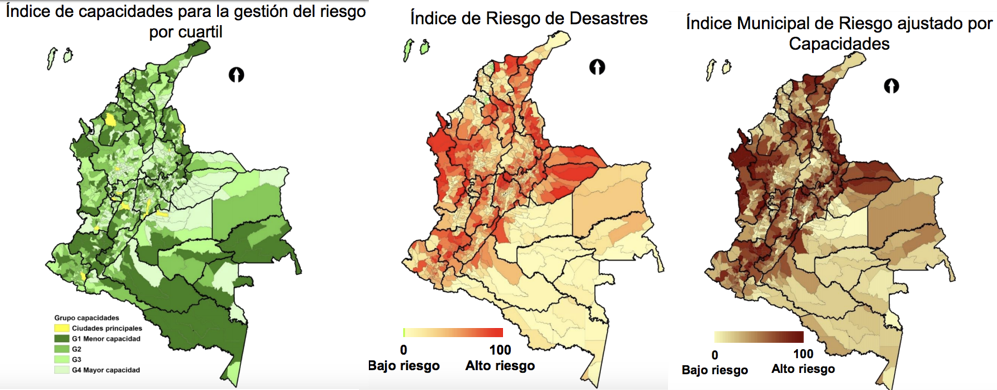
\includegraphics[width=0.95\textwidth]
        {riskIndexesCol}}
        \caption{Risk Management Index of Colombia adjusted on the basis of capacities. The index which is illustrated on the right image combines the capacity of territorial subdivisions to manage the risk (image on the left), and their risk of a disaster (image in the center). Image taken from \cite{DNP2018}}
        \label{fig:riskIndex}
      \end{figure}
  
  
Based on the previously mentioned facts \textbf{in this project} we present the development process of the tool called: \textbf{Integrated Map of Risk Information in Colombia}  which we consider a tool that is a means to an end. It presents key information of the general situation of the country in terms of risk and can be used as a tool to guide future decisions in the different regions.

The following sections describe the steps follow to develop the tool.    

%%%IMPORTANTE AFTER 2012
%Acciones 2012: 
%Modernizo su sstema nacional de gestion de riesgo. 
%Politica nacional de gestion de riesgo de desastres

%2010 y 2016 se invirio en gestion del riesgo de dsstres 3 veces mas que en el periodo 2002  y 2009 esa inversion se concentra a nivel nacional y municipal BAJO departamental


\section{Problem Description}
\label{sec:probl}
However, in this project, we challenged ourselves to present all the data together, in a way that any of us, as citizens, could make a decision, derive a conclusion or even form an opinion about what is happening in the region.

The Municipal Capacities-Adjusted Disaster Risk Index is an innovative indicator for policymakers to make informed decisions about how to better preserve citizens\' well-being in the presence of real and potential threats. However, to be actionable, information needs not only to be available but efficiently delivered to communities, as a mean of protecting citizen\'s rights, foster economic growth, and make government officials accountable. 

As mentioned previously, \textbf{Colombia} already \textbf{has} an index, \textbf{the Risk Management Index of Colombia adjusted on the basis of capacities}. However, official risk management \textbf{information lacks of a understandable delivery system}, that enables local communities \textbf{to improve their risk awareness} and disaster coping capabilities, in scenarios such as extreme temperatures and changing weather patterns.

For instance,  in the official information, \textbf{it is not apparent how similar events have impacted communities with different risk and vulnerability profiles}, and there is no relevant information to assess the performance of risk management activities.  

The decision to choose a topic in the field of \textbf{Risk and Vulnerability to natural disasters} was also based on two main reasons:

\begin{enumerate}

\item Besides any discrepancies people may have in terms of the cause of \textbf{climate change}, most people and the scientific community agree that it \textbf{is happening}. The world is  experiencing changes in temperature patterns worldwide, and that has a direct correlation with the frequency of extreme hydrometeorological events. As it is shown in Figure \ref{fig:globlaEvents}, global temperatures are increasing, and extreme weather events have increased in the last 60 years. In Colombia, the hydrometereological events are responsible of 88\% of the disasters according to \cite{DNP2018}

\begin{figure}%
\centering
\subfigure[Global temperature anomalies]{%
\label{fig:globlaEvents_a}%
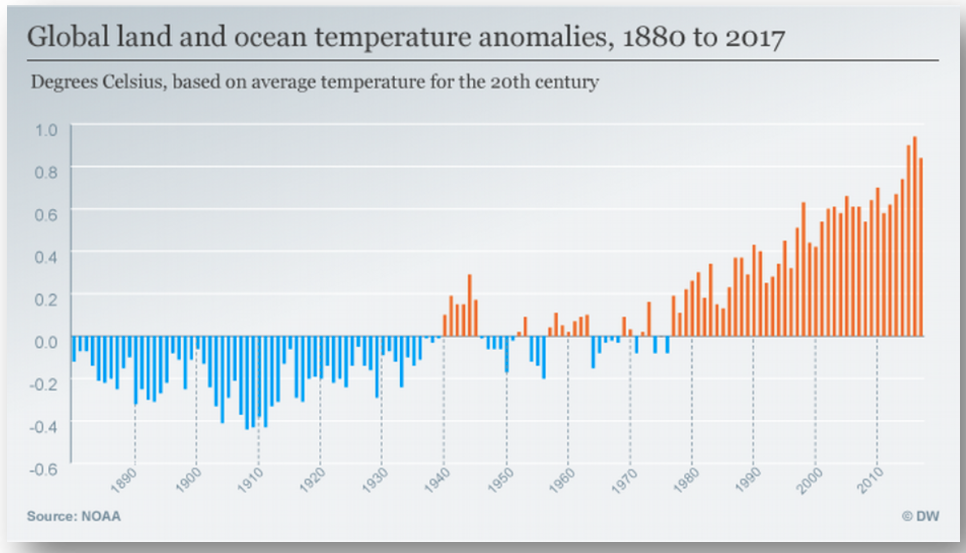
\includegraphics[height=2.5in, width=3in] {temp2.png}}
\qquad
\subfigure[Number of extreme weather events per year]{%
\label{fig:globlaEvents_b}%
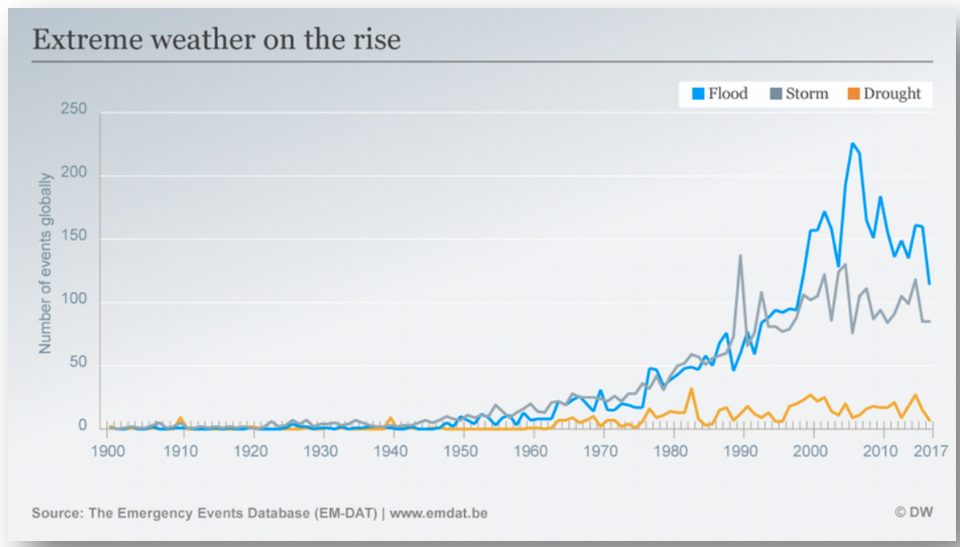
\includegraphics[height=2.5in, width=3in]{temp1.png}}
\caption{Frequency of extreme hydro-meteorologica events.}
\label{fig:globlaEvents}%
\end{figure}

\item The exposition to the effects of such hydrometereological events is not equally distributed. \textbf{Risk from a natural disaster} is somewhat \textbf{random} but \textbf{vulnerability is anthropogenic}. In other words, the cost of two events similar in magnitude, in two different places, can vary from some physical damage, to the loss of vital infrastructure and even human lives.

\end{enumerate}


\section{Proposal}
\label{sec:prop}

With the proposed \textbf{Dashboard Web Application}, the team expects \textbf{to enable any person} to find, read and \textbf{understand the basic risk profile of their region of interest} and also understand about climate associated risks. All this based on open data philosophy.

We set out to do 3 things:

\begin{itemize}
\item Find historic evidence of those claims. 
\item Create an index to capture and monitor that imbalance in the allocation of coping capabilities and resources.
\item Offer actionable information to both the general public and administration officials to improve their understanding of future impact of climatic events.
\end{itemize}

\textbf{Open data} is not just about putting information in the cloud and making it available for people to download it. It is \textbf{a philosophy and practice that guarantees availability for all} in order to use data to foster economic growth, protect citizen's and business' rights, and delimit administration's accountability.

Put in another way: it is not open data if there is a knowledge barrier that keep it out of most people's reach. 




\subsection{Possible use}
\label{sec:prop}


The developed tool could be of value for the people in general, outside our regular interests, activities and industries. Imagine you are a person casting a vote: 

\begin{itemize}
\item The worst equipped your region is to deal with emergencies, the more important is for you to know which candidate is prioritizing those capabilities.
\item If you are an elected official, getting a clear picture of the risk profile of your district at a glance is a core asset when allocating resources, and designing preemptive plans. For instance, knowing that now precipitations level is close to the historical maximum can trigger an early alarm.

\end{itemize}


\section{Datasets sourced }
\label{sec:app}

The main dataset used in the project is from the Colombia Risk of Disaster Management Unit (Unidad de Gesti\'{o}n de Riesgos y Desastres) UNGRD \cite{datasetUNGRD}. The dataset contains information about  the risk management associated with natural phenomena, socio-natural, technologic, and human-based non-intentional incidents reported in Colombia in the last 10 years (38626 records). Some of the fields found in the dataset are: Date, Department, Municipality, Event Name, Code, Dead, Wounded, Disappeared, Affected People, Affected Families, Affected Houses, among others.

The team will also use a dataset from the National Administrative Department for Statistics DANE. It is a time series between 1985 to 2020 and contains demographic information, per department code \cite{DANE} .

Both datasets contain ``DIVIPOLA'' codes, which is the codification of the Politica-Administrative Division of Colombia (Codification of the departments, ). Figure \ref{fig:divipola} describes the meaning of the code. The first two numbers correspond to the department, followed by the Municipality Code and the Populated Center \cite{divipol}.


\begin{figure}[!ht]
        \center{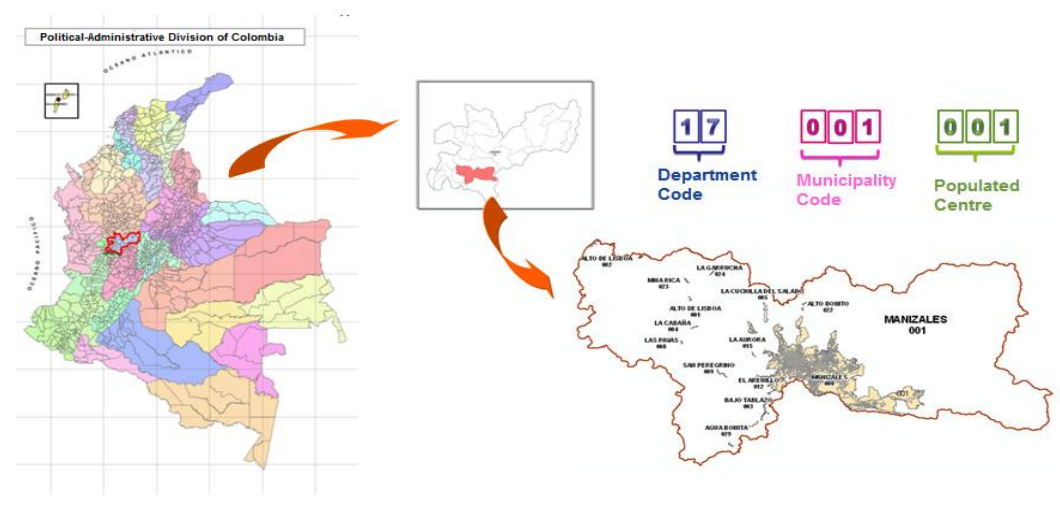
\includegraphics[width=0.8\textwidth]
        {divipolaExplanation}}
        \caption{Explanation of ``DIVIPOLA'' code. The codes provide information of the Politica-Administrative Division of Colombia. Image taken from \cite{divipol}}
        \label{fig:divipola}
      \end{figure}
